\section{Introduction}
\subsection{GPU Programming Language}
\begin{frame}{GPU vs CPU}
\framesubtitle{The CPU}
	\begin{itemize}
        \item Central Processing Unit (CPU)
        \item Sequential serial processing advantage
        \item A small amount of more powerful cores
        \item Affected by Moore’s law
    \end{itemize}
\end{frame}

\subsection{GPU Programming Language}
\begin{frame}{GPU vs CPU}
\framesubtitle{Moore’s law}
  \begin{itemize}
        \item Exponential growth in transistor count
        \item Breakpoint at 2020 or 2022 foresees Intel
    \end{itemize}
    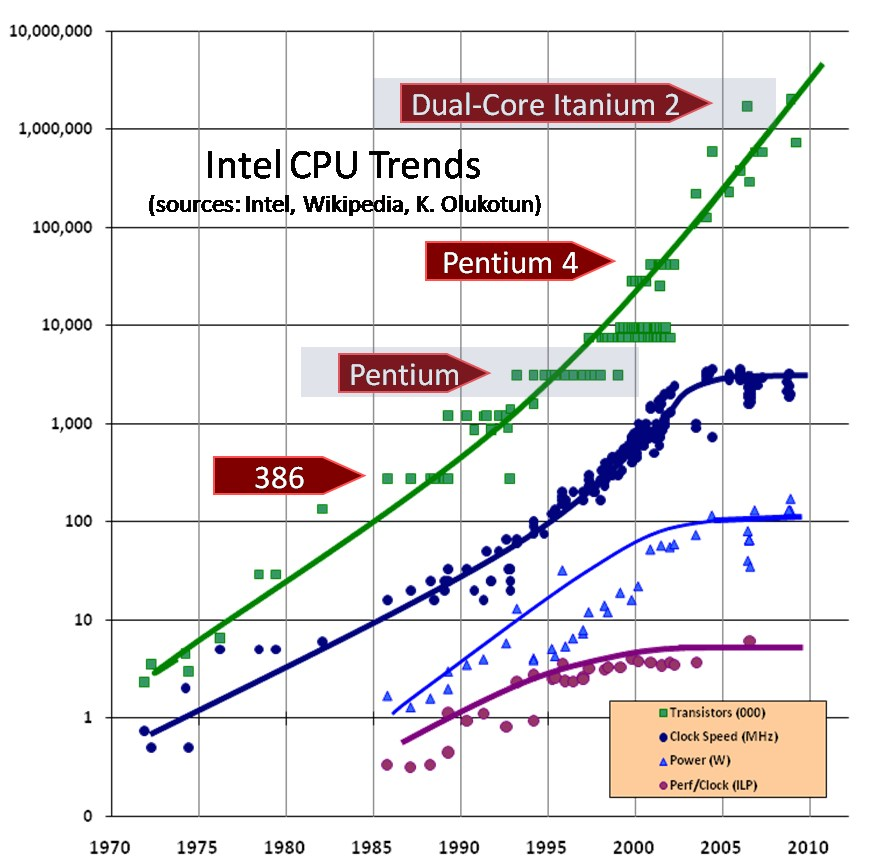
\includegraphics[width=1\textwidth,height=0.7\textheight,keepaspectratio, , clip]{images/CPU-Scaling.jpg}
\end{frame}

\subsection{GPU Programming Language}
\begin{frame}{GPU vs CPU}
\framesubtitle{The GPU}
  \begin{itemize}
        \item Graphics Processing Unit (GPU)
        \item A large amount of less powerful cores
        \item Parallel computing advantage
        \item Hard to program -  large amount of boilerplate
    \end{itemize}
    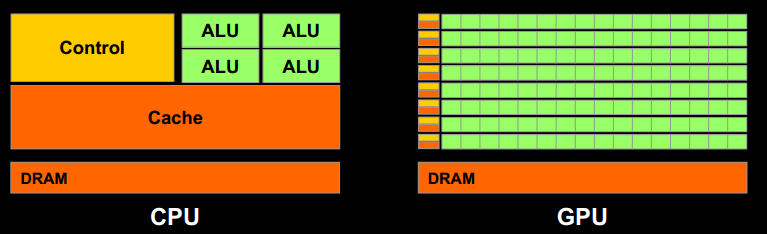
\includegraphics[width=1\textwidth,height=0.7\textheight,keepaspectratio, , clip]{images/GPUCPUimage.png}
\end{frame}

\subsection{GPU Programming Language}
\begin{frame}{GPU vs CPU}
\framesubtitle{Comparison}
  \begin{itemize}
        \item GPU theoretically allows for about 12 times more floating point operations per second
    \end{itemize}
    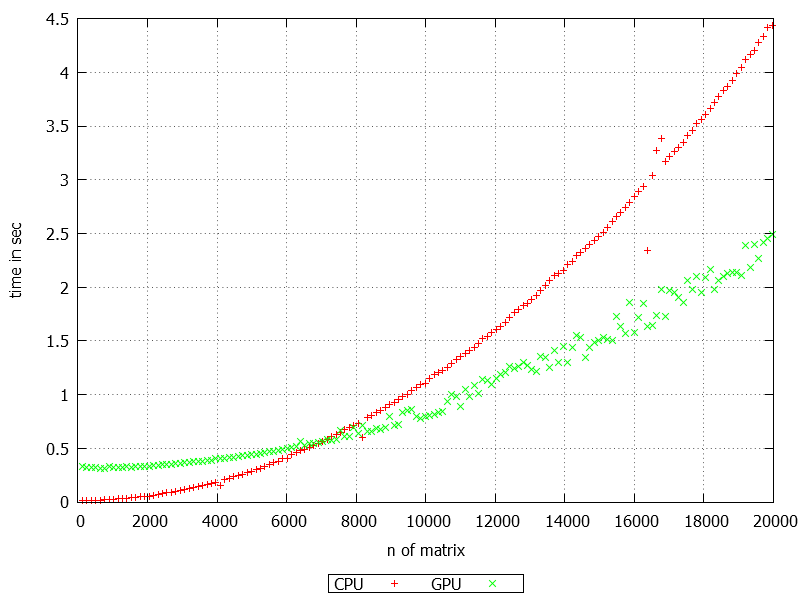
\includegraphics[width=1\textwidth,height=0.7\textheight,keepaspectratio, , clip]{images/benchmark.png}
\end{frame}

\subsection{GPU Programming Language}
\begin{frame}{GPU vs CPU}
\framesubtitle{Example of parallel computation}
  \begin{itemize}
        \item Graphic Processing Unit
        \item Pixels are elements in matrices
        \item Matrices is easy to manipulate in parallel
        \item Linear algebra
    \end{itemize}
    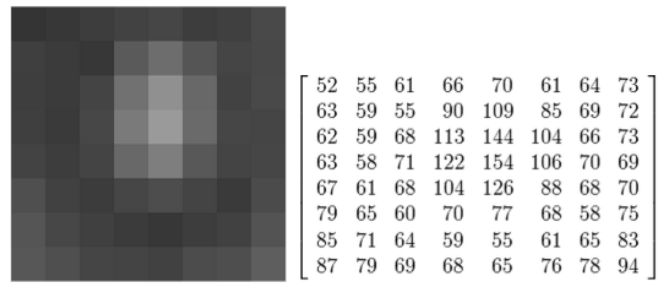
\includegraphics[width=1\textwidth,height=0.7\textheight,keepaspectratio, , clip]{images/matrix_Mat_object.png}
\end{frame}

\subsection{GPU Programming Language}
\begin{frame}{Existing solutions}
\framesubtitle{Table }
  %\begin{table}
	\centering
    \colorlet{shadecolor}{gray!40}
    \rowcolors{1}{white}{shadecolor}
	\begin{tabular}{|l|c|c|l|l|}
	\hline
	\textbf{Language} & \textbf{CUDA}         & \textbf{OpenCL} & \textbf{Abstraction} & \textbf{Comment}			  		\\ \hline
	Theano   & \cmark           & \cmark            & High      &  Native                                                          \\ \hline
	Matlab   & \cmark           & \cmark            & Low/High        &  \gls{opencl} via extensions, \gls{cuda} is native                                                         \\ \hline
	Julia    & \cmark           & \cmark              & High        &  Both via extensions                                                          \\ \hline
	R        & \cmark           & \cmark            & Low/High    & Abstraction is depended on the use of either \gls{cuda} or \gls{opencl} \\ \hline
	C   & \cmark           & \cmark            & Low         & via \gls{cuda} C, and \gls{opencl} C (Both are supersets of C)                                           \\ \hline
	Java     & \cmark           & \cmark              &   Low          & Bindings such as jcuda and jocl                                            \\ \hline
	\end{tabular}
	\caption{Existing GPU supporting languages. }\label{tbl:sota}
\end{table}
                
\end{frame}

\subsection{GPU Programming Language}
\begin{frame}{Problem statement}
\framesubtitle{Problem statement}
\[
  \left[
  \begin{minipage}{\textwidth}
  \centering
  \begin{minipage}{0.96\textwidth}
  How does one design a programming language, with a corresponding compiler or interpreter, which compiles source code to execute on the gpu at runtime for certain linear algebra calculations, such as matrix operations?
  \end{minipage}
  \end{minipage}
    \right]
\]
\end{frame}